% !TEX program = xelatex
\documentclass[hyperref,a4paper,UTF8]{ctexart}

\usepackage[left=2.50cm, right=2.50cm, top=2.50cm, bottom=2.50cm]{geometry}

\usepackage[unicode=true,colorlinks,urlcolor=blue,linkcolor=blue,bookmarksnumbered=true]{hyperref}
\usepackage{latexsym,amssymb,amsmath,amsbsy,amsopn,amstext,amsthm,amsxtra,color,bm,calc,ifpdf,booktabs}
\usepackage{graphicx}
\usepackage{enumerate}
\usepackage{fancyhdr}
\usepackage{listings}
\usepackage{multirow}
\usepackage{makeidx}
\usepackage{xcolor}
\usepackage{fontspec}
\usepackage{subfigure}
\usepackage{hyperref}
\usepackage{pythonhighlight}
\usepackage[ruled,linesnumbered]{algorithm2e}


\pagestyle{fancy}
\fancyhead[L]{}
\fancyhead[C]{\fangsong 云南大学信息学院机器学习实验(2023春)课程论文}
\fancyhead[R]{}

\renewcommand{\abstractname}{\textbf{\large {摘\quad 要}}} % 更改摘要二字的样式


\title{
机器学习实验(2023春)课程论文\\
~\\
\textbf{基于多种方式实现的中国手游行业满意度分析}
}
\author{
\kaishu\normalsize
姓名\ \underline{李昂} \qquad
学号\ \underline{20201060287} \qquad
}
\date{} % 留空,不显示日期


\begin{document}

\begin{figure}
    \centering
    
\includegraphics[width=0.7\textwidth]{fig/ynu.jpg}
\end{figure}

\maketitle



\begin{abstract}
随着社交媒体和在线平台的普及,用户对产品、服务和事件的评价越来越多地以文字形式表达。这些用户生成的文本数据蕴含着丰富的情感信息,包括积极的评价、负面的抱怨、中立的观点等,对于了解用户需求、改进产品质量、推动市场营销等方面具有重要意义。


为了挖掘和分析这些海量的Web文本数据,情感分析成为一项关键技术。情感分析的目标是通过自然语言处理和机器学习技术,自动识别和分类文本中的情感倾向,如正面、负面或中性。这项技术的应用范围广泛,不仅限于用户评论,还包括社交媒体上的帖子、新闻报道、市场调研数据等。本实验依据中文游戏平台Taptap用户的评论,分析中国手游用户对手机游戏的满意度。


本文以文本颗粒度为视角,对情感分析的研究对象和目标进行了定义和说明。然后在句子级别的识别任务上详细回顾和分析了主要的处理方法:基于语义的情感词典分类方法、基于机器学习的情感分类方法、基于深度学习的情感分类方法和基于迁移学习的情感分类方法学习,并提出了未来的研究方向。

\end{abstract}
\thispagestyle{empty} % 当前页不显示页码

\newpage

\tableofcontents
\thispagestyle{empty} % 当前页不显示页码

\newpage

\listoffigures
\listoftables


\thispagestyle{empty} % 当前页不显示页码
\newpage


\section{引言}

互联网的快速发展促进了其自身由“阅读式互联网”向“交互式互联网”转变。网络不仅成为人们获取信息的重要来源,也成为人们发表自己的观点和分享自己的体验,直接表达喜、怒、哀、乐等各种情感的重要平台。 


当前,针对网络文本内容的处理技术主要着眼于客观性信息,相应信息检索一般为关键词检索,信息抽取技术主要抽取文本描述的特定事件发生的时间、地点、相关人物、过程、属性等,信息抽取结果大多是客观性事实,并按照客观主题进行分类。面对大量来自微博、论坛、博客的非结构化或半结构化评论文本,迫切需要通过计算机快速、有效地完成意见性文本信息分类和情感信息的抽取,然后通过挖掘和分析文本中的立场 、观点 、看法、情绪 、好恶等主观信息 ,对文本的情感倾向做出判断。 \cite{DBLP:journals/ijon/MerchaB23}

\section{情感语义分析综述}

\subsection{情感分析简述}

\textit{文本情感分析(Sentiment Analysis)是指利用自然语言处理和文本挖掘技术,对带有情感色彩的主观性 文本进行分析、处理和抽取的过程。}

\begin{figure}[ht]
	\centering
	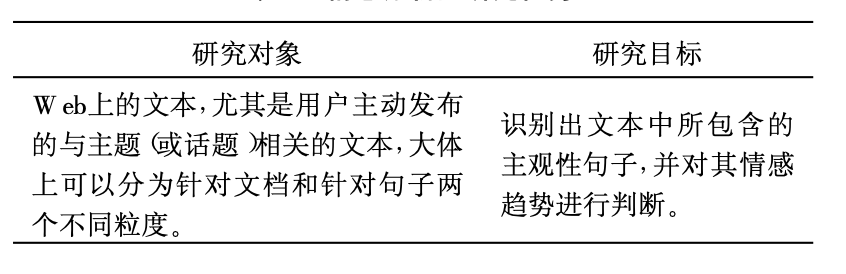
\includegraphics[width=0.8\textwidth]{fig/pic1.png}
	\caption{情感分析的研究任务}
    \label{fig:example}
\end{figure}

目前,文本情感分析研究涵盖了包括自然语言处理、文本挖掘、信息检索、信息抽取、机器学习和本体学等多个领域,得到了许多学者以及研究机构的关注,近几年持续成为自然语言处理和文本挖掘领域研究的热点问题之一。情感分析任务按其分析的粒度可以分为篇章级,句子级,词或短语级; 按其处理文 本的类别可分为基于产品评论的情感分析和基于新闻评论的情感分析; 按其研究的任务类型,可分情 感分类,情感检索和情感抽取等子问题。 \cite{DBLP:journals/ijon/MerchaB23}


文本情感分析的基本流程如图 1 所示,包括从原始文本爬取,文本预处理,语料库和情感词库构建以及 情感分析结果等全流程。由于文本原始素材爬取、分词等预处理技术已比较成熟,本文接下来将通过情感分析的主要任务情感分类,来分析和阐述相关研究工作。

\begin{figure}[ht]
	\centering
	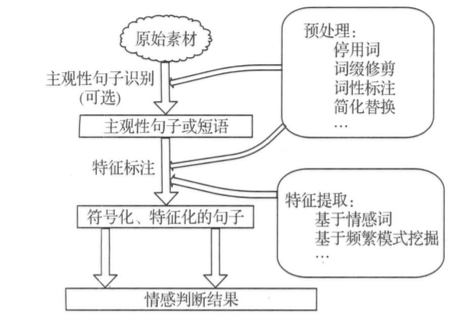
\includegraphics[width=0.8\textwidth]{fig/pic2.png}
	\caption{情感分析的基本流程}
    \label{fig:example}
\end{figure}


\subsection{情感分类}
\textit{情感分类又称情感倾向性分析,是指对给定的文本,识别其中主观性文本的倾向是肯定还是否定的,或者说是正面还是负面的,是情感分析领域研究最多的。} \cite{DBLP:journals/ijon/MerchaB23}



通常网络文本存在大量的主观性文本和客观性文本。客观性文本是对事物的客观性描述,不带有感情色彩和情感倾向,主观性文本则是作者对各种事物的看法或想法,带有作者的喜好厌恶等情感倾向。情感分类的对象是带有情感倾向的主观性文本,因此情感分类首先要进行文本的主客观分类。文本的主客观分类主要以情感词识别为主,利用不同的文本特征表示方法和分类器进行识别分类,对网络文本事先进行主 客观分类,能够提高情感分类的速度和准确度。


纵观目前主观性文本情感倾向性分析的研究工作,主要研究思路分为基于语义的情感词典方法、基于机器学习的方法和基于深度学习的方法。
\subsubsection{基于语义的情感词典方法}

基于情感词典的情感语义分析是一种通过使用预先构建好的情感词典来判断文本中每个词的情感极性,并进一步通过计算来推断整个文本的情感倾向。该方法将文本按照情感词汇进行词汇匹配,并对每个匹配到的情感词赋予一个情感极性值,然后通过对这些极性值进行求和或平均来得出整体情感倾向。这种方法简单高效,适用于大规模情感分析的任务。\cite{DBLP:journals/widm/ZhangWL18}

\subsubsection{基于机器学习的情感分类方法}

基于机器学习的情感语义分析是利用机器学习算法对文本进行自动分析和理解,从中提取出情感和语义的信息。它包括训练模型来对文本进行分类,将其划分为情感类别(如正面、负面、中性)以及语义类别(如人物、地点、事件),以实现对文本情感和意义的自动化理解和处理。这种方法可以应用于社交媒体监测、产品评论分析、舆情分析等领域,帮助人们快速了解大量文本的情感倾向和语义信息。\cite{DBLP:journals/widm/ZhangWL18}

\subsubsection{基于深度学习的情感词典方法}

基于深度学习的情感语义分析是利用深度学习算法处理文本数据,通过训练模型来识别文本中的情感信息和语义关系。它能够对文本进行自动情感分类、情感极性判断、情感强度评估等任务,有助于理解和应用自然语言中的情感表达。


特别的,基于迁移学习的情感语义分析是一种利用已有知识和模型来处理情感分类任务的方法。通过从一个源领域学习到的模型和知识,将其应用于目标领域的情感语义分析任务中,可以提高目标领域情感分类的性能。这种方法可以避免从头开始训练模型的问题,节省时间和计算资源,并且可以在数据量不足的情况下获得更好的结果。


\section{实验内容与结果}

\subsection{基于语义的情感词典方法}

\subsubsection{概述}

(1)构建词典


情感词典的构建是情感分类的前提和基础,目前在实际使用中,可将其归为 4 类:通用 情感词、程度副词、否定词、领域词。目前国内外,情感词典的构建方法主要是利用已有电子词典扩展生成情感词典。英文方面主要是基于对英文词WordNet 的扩充,中文方面则主要是对知网 Hownet 的扩充。此外,还可以建立专门的领域词典,以提高情感分类的准确性。


(2)构建倾向性计算算法


基于语义的情感词典的倾向性计算不同于所需大量训练数据集的机器学习算法,主要是利用情感词典及句式词库分析文本语句的特殊结构及情感倾向词,采用权值算法代替传统人工判别或仅利用简单统计的方法进行情感分类。给情感强度不同的情感词赋予不同权值,然后使用公式(1)加权求和。

 \begin{equation}
\bar{E}=\frac{\sum_{i=1}^{N_p} \mathrm{wp}_i+\sum_{j=1}^{N_n} \mathrm{wp}_j}{N_p+N_n}
\end{equation}


(3)确定阈值来判断文本倾向性

一般情况下,加权计算结果为正是正面倾向,结果为负是负面倾向,得分为零无倾向。所得结果评价一般采用自然语言中 经常使用的正确率、召回率和 F 值来评判算法效果。


基于情感词典的方法和基于机器学习的分类算法相比,虽属于粗粒度的倾向性分类方法,但由于不依赖标注好的训练集,对于普遍通用领域的网络文本可有效快速地进行情感分类。

\subsubsection{实验结果}

本次试验采用了BosonNLP提供的情感词典。


BosonNLP情感词典是从微博、新闻、论坛等数据来源的上百万篇情感标注数据当中自动构建的情感极性词典。因为标注包括微博数据,该词典囊括了很多网络用语及非正式简称,对非规范文本也有较高的覆盖率。该情感词典可以用于构建社交媒体情感分析引擎,负面内容发现等应用。


在BosonNLP情感词典中,文本采用UTF-8进行编码,每行为一个情感词及其对应的情感分值,以空格分隔,共包括114767个词语。其中负数代表偏负面的词语,非负数代表偏正面的词语,正负的程度可以由数值的大小反应出。

\begin{table}[ht]
    \centering
    \begin{tabular}{c|lr} % 通过添加 | 来表示是否需要绘制竖线
        \toprule
        词语 & 情感值\\
        \midrule
        爱死了  & +6.70400012637\\
        \hline  %在第一行和第二行之间绘制横线
        扰民  & -6.49756445867 \\
        \hline  %在第二行和第三行之间绘制横线
        吃哑巴亏  & -5.77120419579 \\
        \bottomrule
    \end{tabular}
    \caption{BosonNLP示例}
    \label{tab:example}
\end{table}

使用情感词典分类,精度为64.13\%。

\subsection{基于机器学习的方法}
\textit{文本情感倾向性分析与传统的基于主题的文本分类相似但有所不同,基于主题的文本分类是把文本分 类到各个预定义的主题上,如军事,互联网,政治,体育 等,而情感分类不是基于内容本身的,而是按照文本持 有的情感、态度进行判断。现有任何机器学习的分类 方法都可以用到情感分类中来。基于机器学习的情感 分类,其大致流程如下:首先人工标注文本倾向性作为 训练集,提取文本情感特征,通过机器学习的方法构造 情感分类器,待分类的文本通过分类器进行倾向性分类。}\cite{DBLP:journals/widm/ZhangWL18}


\subsubsection{贝叶斯分类器}

\textbf{概述}

贝叶斯分类器是一种基于贝叶斯定理的概率模型,用于进行分类任务。它假设样本的特征是条件独立的,并利用训练数据中的类别和特征之间的概率关系,计算出后验概率,然后基于后验概率进行分类。
\cite{DBLP:journals/corr/abs-1801-07883}


1. 根据贝叶斯定理,我们有:
   $ P(c|x) = \frac{P(x|c) \cdot P(c)}{P(x)} $

   其中,$ P(c|x) $ 是后验概率,表示在给定特征 $ x $ 的情况下类别 $ c $ 的概率;$ P(x|c) $ 是似然概率,表示在类别 $ c $ 的情况下特征 $ x $ 的概率;$ P(c) $ 是先验概率,表示类别 $ c $ 的概率;$ P(x) $ 是证据因子,表示特征 $ x $ 的概率。

2. 由于我们的目标是找到后验概率最大的类别 $ c_{\text{max}} $,我们可以忽略证据因子 $ P(x) $,因为它对于所有类别都是相同的,不会影响最大后验概率的比较。

3. 进一步简化,我们可以假设样本的特征是条件独立的,即:
   $ P(x|c) = P(x_1|c) \cdot P(x_2|c) \cdot ... \cdot P(x_n|c) $

   其中,$ x_1, x_2, ..., x_n $ 是样本的特征。

4. 最终的分类器可以表示为:
   $ c_{\text{max}} = \text{argmax}_c P(c) \cdot \prod_{i=1}^n P(x_i|c) $

   其中,$ \text{argmax}_c $ 表示使得后面表达式最大化的类别 $ c $。

利用训练数据估计先验概率和似然概率,然后应用分类器以对新的样本进行分类。


\textbf{实验结果}


使用朴素贝叶斯分类器进行分类,精度为65.21\%。
\subsubsection{支持向量机}

\textbf{概述}


Support Vector Machine (SVM) 是一种常用的监督学习算法,用于解决分类和回归问题。它的主要思想是将数据集映射到高维空间,然后在该空间中找到一个最优的超平面来进行分类。这个超平面能够最大化训练样本与超平面之间的间隔,从而使得分类更加准确。\cite{DBLP:journals/corr/abs-1801-07883}


1. 假设我们有一组已标记的训练样本 $D = \{(x_1, y_1), (x_2, y_2), ..., (x_n, y_n)\}$,其中 $x_i$ 是输入特征向量,$y_i$ 是对应的类别标签,可以取值为 -1 或 1。

2. 我们希望找到一个超平面 $w \cdot x + b = 0$,其中 $w$ 是法向量,$b$ 是偏置项。

3. 对于任意样本点 $(x_i, y_i)$,有以下约束条件:
   - 如果 $y_i = 1$,则要求 $w \cdot x + b \geq 1$,即样本点位于超平面正类别一侧的间隔边界内部。
   - 如果 $y_i = -1$,则要求 $w \cdot x + b \leq -1$,即样本点位于超平面负类别一侧的间隔边界内部。

4. 根据约束条件,我们可以得到以下优化问题:
   $$\text{minimize} \;\; \|w\|$$
   $$\text{subject to} \;\; y_i(w \cdot x_i + b) \geq 1 \;\; \text{for all} \;\; (x_i, y_i) \in D$$

5. 进一步转化为拉格朗日对偶问题:
   $$\text{maximize} \;\; L(\alpha) = \sum_{i=1}^{n}\alpha_i - \frac{1}{2}\sum_{i=1}^{n}\sum_{j=1}^{n}\alpha_i\alpha_jy_iy_jx_i\cdot x_j$$
   $$\text{subject to} \;\; \sum_{i=1}^{n}\alpha_iy_i = 0 \;\; \text{and} \;\; \alpha_i \geq 0 \;\; \text{for all} \;\; i$$

6. 对拉格朗日函数求导,并令导数为零,得到下面的等式:
   $$w = \sum_{i=1}^{n}\alpha_iy_ix_i$$

7. 根据 Karush-Kuhn-Tucker(KKT)条件,我们可以得到以下结果:
   $$\alpha_i(y_i(w \cdot x_i + b) - 1) = 0 \;\; \text{for all} \;\; i$$

8. 最终,可以得到超平面为:
   $$w \cdot x + b = \sum_{i=1}^{n}\alpha_iy_ix_i \cdot x + b = 0$$

\textbf{实验结果}


使用支持向量机器做分类器,精度为62.49\%。

\subsubsection{AdaBoost}

\textbf{概述}

Adaboost (Adaptive Boosting)是一种常见的集成学习算法。它通过训练一系列弱分类器来构建一个强分类器。Adaboost的伪代码如下:

输入:训练数据集 $\{(x_1,y_1), (x_2,y_2), ..., (x_N,y_N)\}$,其中 $x_i$ 是输入特征向量,$y_i$ 是标签(分类结果)。

输出:最终的分类器 $H(x)$。

1. 初始化样本权重 $D_1(i) = \frac{1}{N}, \ i = 1,2,...,N$。

2. 对于 $t = 1,2,...,T$(迭代次数,$T$ 是弱分类器的个数):

    a. 使用当前权重 $D_t(i)$ 来训练一个弱分类器 $G_t(x)$。
    
    b. 计算弱分类器 $G_t(x)$ 的误差率 $\varepsilon_t = \sum_{i=1}^{N} D_t(i) \cdot \mathbb{I}(G_t(x_i) \neq y_i)$,其中 $\mathbb{I}$ 是指示函数。
    
    c. 计算弱分类器的权重 $\alpha_t = \frac{1}{2} \ln \left( \frac{1-\varepsilon_t}{\varepsilon_t} \right)$。
    
    d. 更新样本权重 $D_{t+1}(i) = \frac{D_t(i) \cdot \exp(-\alpha_t y_i G_t(x_i))}{Z_t}$,其中 $Z_t$ 是规范化因子,使得 $D_{t+1}(i)$ 成为一个概率分布。
    
3. 输出最终的分类器 $H(x) = \text{sign} \left( \sum_{t=1}^{T} \alpha_t G_t(x) \right)$。

\textbf{实验结果}


使用AdaBoost集合朴素贝叶斯和支持向量机两种分类器,精度为64.28\%。

\subsection{基于深度学习的方法}

\subsubsection{概述}
\textit{深度学习是一种机器学习方法,其基本思想是模拟人类神经网络的工作原理,通过多层次的神经网络结构来学习和提取数据的特征。它是由许多神经元之间的连接和权重调整而构成的,通过大量的训练数据来优化网络参数,以便进行分类、回归、聚类等任务。深度学习在计算机视觉、自然语言处理、语音识别等领域取得了重要的突破。}\cite{DBLP:journals/corr/abs-1801-07883}


反向传播(Backpropagation,BP)算法是深度学习中最常用的优化方法之一。它通过计算损失函数对每个参数的梯度,然后利用梯度下降的方法来更新参数,从而使得模型能够逐步优化。

BP算法的核心思想是利用链式法则来计算参数的梯度。具体而言,它首先通过前向传播计算模型的输出,然后通过反向传播计算每个参数对损失函数的梯度,最后利用梯度下降法来更新参数。首先,定义神经网络模型的输入为$\mathbf{x}$,输出为$\mathbf{y}$。模型的预测输出为$\hat{\mathbf{y}}$,可以表示为:

$$\hat{\mathbf{y}} = \mathbf{f}(\mathbf{W}_2 \mathbf{h})$$

其中,$\mathbf{W}_2$是模型的权重参数,$\mathbf{h}$是隐藏层的输出,$\mathbf{f}$是激活函数。

接下来,定义模型的损失函数为$L$,通常采用均方差(Mean Squared Error):

$$L = \frac{1}{2} \Vert \mathbf{y} - \hat{\mathbf{y}} \Vert^2$$

为了更新模型的权重参数,需要求解损失函数关于权重参数的梯度。根据链式法则,可以得到:

$$\nabla_{\mathbf{W}_2} L = (\mathbf{y} - \hat{\mathbf{y}}) \odot \mathbf{f}'(\mathbf{W}_2 \mathbf{h}) \mathbf{h}^T$$

其中,$\nabla_{\mathbf{W}_2} L$表示关于$\mathbf{W}_2$的梯度,$\mathbf{h}^T$表示$\mathbf{h}$的转置。

进一步,定义$\mathbf{e} = (\mathbf{y} - \hat{\mathbf{y}}) \odot \mathbf{f}'(\mathbf{W}_2 \mathbf{h})$,则可以简化梯度的表达式为:

$$\nabla_{\mathbf{W}_2} L = \mathbf{e} \mathbf{h}^T$$

接下来,继续求解关于隐藏层的梯度。定义$\mathbf{d} = \mathbf{W}_2^T \mathbf{e} \odot \mathbf{f}'(\mathbf{W}_1 \mathbf{x})$,则隐藏层的梯度可以表示为:

$$\nabla_{\mathbf{W}_1} L = \mathbf{d} \mathbf{x}^T$$

最后,通过梯度下降法更新权重参数$\mathbf{W}_1$和$\mathbf{W}_2$:

$$\mathbf{W}_1 \leftarrow \mathbf{W}_1 - \alpha \nabla_{\mathbf{W}_1} L$$
$$\mathbf{W}_2 \leftarrow \mathbf{W}_2 - \alpha \nabla_{\mathbf{W}_2} L$$

其中,$\alpha$是学习率,用于控制参数更新的步长。


通过反复迭代运用BP算法,深度学习模型可以不断地优化,从而在大规模数据上实现更好的学习和预测效果。

\subsubsection{Bi-LSTM}
\textbf{简介}


Bi-LSTM(双向长短期记忆网络)是一种循环神经网络(RNN)的变体,用于处理序列数据。与传统的单向LSTM不同,Bi-LSTM通过在前向和后向同时运行两个LSTM层来捕捉序列中的上下文信息。前向LSTM从序列的起始位置开始处理,而后向LSTM则从序列的结束位置开始处理。最终,Bi-LSTM通过合并这两个层的输出来得到最终的表示。这种双向的设计使得Bi-LSTM能够同时利用当前位置之前和之后的上下文信息,更好地捕捉序列的特征。Bi-LSTM广泛应用于自然语言处理(NLP)领域,如文本分类、命名实体识别和机器翻译等任务。\cite{DBLP:journals/access/WangWZ23}

\begin{figure}[ht]
	\centering
	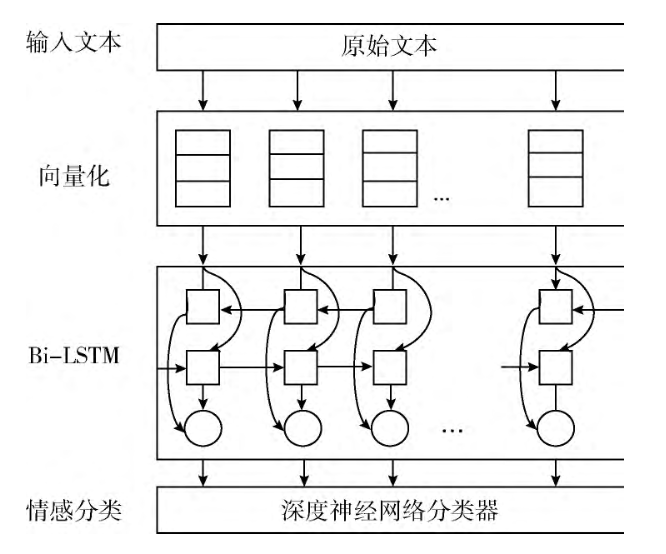
\includegraphics[width=0.5\textwidth]{fig/pic3.png}
	\caption{Bi-LSTM}
    \label{fig:example}
\end{figure}

\newpage

\textbf{实验结果}

\begin{table}[ht]
    \centering
    \begin{tabular}{c|lr}
        \toprule
        \textbf{Hyperparameter} & \textbf{Value} \\
        \midrule
        Test Size & 0.3 \\
        Max Length & 100 \\
        Embedding Dimension & 100 \\
        Hidden Units & 64 \\
        Loss Function & Binary Crossentropy \\
        Optimizer & Adam \\
        Epochs & 50 \\
        Batch Size & 64 \\
        \bottomrule
    \end{tabular}
    \caption{超参数设置和网络详情}
    \label{tab:hyperparameters}
\end{table}

使用Bi-LSTM分类精度为74.15\%。


\subsubsection{LSTM-Attention}


\textbf{简介}


注意力机制来源于人的视觉处理过程,通过浏览全部信息来获得视觉注意力焦点,提取句子所表达信息的主要部分来获取句子中对于当前任务的关键信息。


Atention函数本质上是一个由诸多 Query和 Key-value 组 成 的 映 射 函 数 。 其 计 算 过 程 主 要 分 为 以下三步:


1. 将 query 和每个 key 进行相似度计算得到相应权重 ,如式(2)所示 
    \begin{equation}
    f(Q, K)=Q K^T
    \end{equation}

    
2. 使用 softmax 函数对权重进行归一化


3. 将权重和相应的键值value进行加权求和得到最后的Atention值,如式(4)所示
    \begin{equation}
    \Lambda \text { ttention }(Q, K, V)=\sum a_i V
    \end{equation}
 其中,Q 代表查询,K-V 是文本向量键值对。


\begin{figure}[ht]
	\centering
	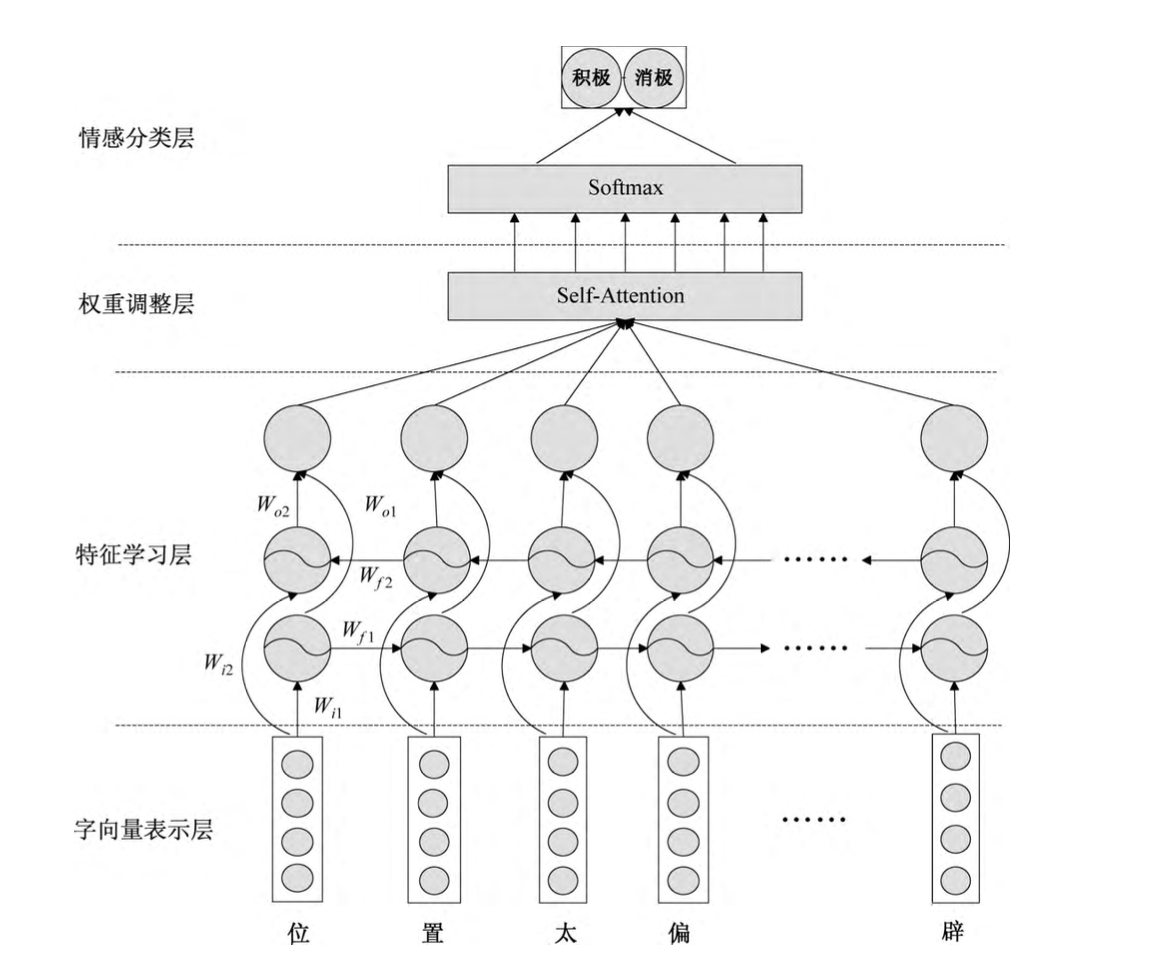
\includegraphics[width=0.6\textwidth]{fig/pic4.png}
	\caption{LSTM with Attention}
    \label{fig:example}
\end{figure}

\textbf{实验结果}


\begin{table}[ht]
    \centering
    \begin{tabular}{c|lr}
        \toprule
        \textbf{Hyperparameter} & \textbf{Value} \\
        \midrule
        Test Size & 0.3 \\
        Max Length & 100 \\
        Embedding Dimension & 100 \\
        Hidden Units & 64 \\
        Loss Function & Binary Crossentropy \\
        Optimizer & Adam \\
        Epochs & 50 \\
        Batch Size & 64 \\
        \bottomrule
    \end{tabular}
    \caption{模型参数表}
    \label{tab:hyperparameters}
\end{table}

使用注意力机制的LSTM,分类精度为69.83\%。


\subsubsection{Finetune-Bert}
\textbf{简介}


BERT(Bidirectional Encoder Representations from Transformers)是一种基于Transformer架构的预训练语言模型。它通过在大规模文本数据上进行无监督训练,学习到丰富的语义表示,可以用于多种自然语言处理任务。Fine-tuning是指在预训练的BERT模型基础上,将其参数进一步微调(fine-tune)以适应特定的任务,比如文本分类、问答系统等。通过这种方式,BERT可以提供更好的性能和泛化能力,适应不同的自然语言处理任务需求。\cite{DBLP:journals/access/UvegesR23}

\newpage

\begin{figure}[ht]
	\centering
	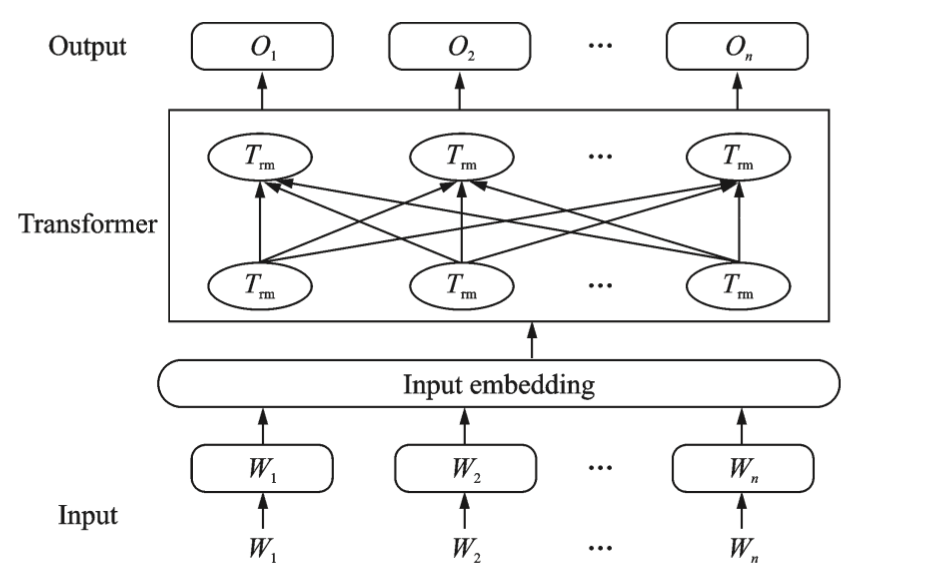
\includegraphics[width=0.6\textwidth]{fig/pic5.png}
	\caption{Bert 结构图}
    \label{fig:example}
\end{figure}

\textbf{实验结果}

\begin{table}[ht]
    \centering
    \begin{tabular}{c|lr}
        \toprule
        \textbf{Hyperparameter} & \textbf{Value} \\
        \midrule
        Batch Size & 16 \\
        Number of Epochs & 5 \\
        Learning Rate & 2e-5 \\
        \bottomrule
    \end{tabular}
    \caption{模型参数表}
    \label{tab:hyperparameters}
\end{table}

使用Bert模型微调,精度为81.07\%。


\section{结果汇总与分析}

\subsection{实验结果汇总}

\begin{table}[ht]
    \centering
    \begin{tabular}{c|lr} % 通过添加 | 来表示是否需要绘制竖线
        \toprule
        分类器 & 精度\\
        \midrule
        情感词典 & 64.13\% \\
        \hline  
        朴素贝叶斯 & 65.21\% \\
        \hline  
        支持向量机 & 62.49\% \\
        \hline  
        AdaBoost & 64.28\%  \\
        \hline  
        Bi-LSTM & 74.15\%  \\
        \hline  
        Attention-LSTM & 69.83\%  \\
        \hline  
        Finetuned-Bert & 81.07\%  \\
        \hline  
        \bottomrule
    \end{tabular}
    \caption{实验结果汇总}
    \label{tab:example}
\end{table}

\subsection{结果分析}

使用情感词典和传统机器学习方法的精度一般,采用深度学习的方式精度提升明显,但也没能达到满意的精度。这可能与数据集的选择有关。

\section{结语}

本次实验采用了多种方法,系统的完成了句级颗粒度的情感语义分析,对于自然语言处理有了更深入的理解。











\newpage
\bibliographystyle{acm}
\bibliography{reference}


\end{document}